

%\section{Experiment Definition}\label{sec:definition}
%The definition of this experiment is following the GQM (Goal - Questions - Metrics) approach \cite{Basili:1992:SMM:137076}. In this section we define the goal of our experiment, the research questions, and the metrics used to answer those questions.



%\begin{table}[h!]
%\centering
%\begin{tabular}{|c|} 
%\hline
%\textbf{Experiment Goal Definition}
%\hline
%Analyze \textbf{Mobile apps \& Web apps} \\ 
%For the purpose of \textbf{Evaluation} \\
%With respect to their \textbf{Energy efficiency }\\
%From the point of view of \textbf{Software developer}\\
%In the context of \textbf{5-20 apps usage of phone and browser}\\ [1ex] 
%\hline
%\end{tabular}
%\caption{Experiment goal of GQM}
%\label{tab:goal}
%\end{table}
%\subsection{Goal}
Based on the GQM definition pattern,the experiment goal is defined on Table 1. The goal is to evaluate apps energy consumption between mobile version and web version. Software developers choose 5 popular apps (up to 20) to monitor energy efficiency. The configuration of the devices type operated by low-end and high-end devices. Web version apps are all operated on Google Chrome.

The principle of choosing the apps depend on %SUGGESTION by Robert: popularity of the application (in the Netherlands) measured by the number of downloads and suggestions given by Google Play, supplemented with some critical thinking about the variety of applications.
The first five options are Facebook,  Twitter, Youtube, Instagram, Google Maps. However, we also prepare alternative 15 apps (NS, Yelp, Skype, Tinder, Weather, Gmail, Amazon, Ebay, NOC, Paypal, Ibooks, ESPN , Netflix, Duolinguo, Uber) to make sure collecting sufficient data in the experiment. Every apps version are the newest.

We want to analyze ..(phone apps and browser apps).. for the purpose of..(evaluation).. with respect to their..(Energy efficiency).. from the point of view of ..(software developer).. in the context of..(Phone usage / thirty phone applications)..?

\subsection{Questions}
Our research embraces 2 research questions: 1 main research question (\textbf{RQ1}), and 1 additional research question (\textbf{RQ2}). The second question will be explored on the condition that there is enough time.

\textbf{RQ1} - How does energy efficiency differ between native mobile applications and their mobile web counterparts?

To answer to this question, we will have to run the same scenarios on pairs consisting of a native mobile application and its mobile web counterpart. Statistical analysis will be performed to determine whether there is any statistically significant difference.

$H_0^1$ - There's no difference in energy efficiency between native mobile applications and their mobile web counterparts.

\textbf{RQ2} - How does the device type (high-end vs low-end) affect the difference in energy consumption between native mobile applications and their mobile web counterparts?

To answer this question, we will have to perform 2 sets of experiments described in \textbf{RQ2}, but one of them has to be on a low-end device, and the other one on a high-end device. Statistical analysis will be performed to determine whether there is any statistically significant difference.

$H_0^2$ - The device type (high-end vs low-end) does not influence the difference in energy consumption between native mobile applications and their mobile web counterparts.

\subsection{Metrics}
We will use the following 4 metrics to answer our research questions. The last one, \textbf{energy efficiency}, is what we will directly use to answer our research questions.

\textbf{Power consumption (W)} - average power consumption of a scenario measured using Trepn Power Profiler \cite{trepn}.

\textbf{Running time (s)} - total running time of a scenario.

\textbf{Energy consumption (J)} - total energy consumed by running a scenario. Calculated by multiplying the average power consumption and the running time of a scenario.

\textbf{Energy efficiency} - ratio of energy consumed by a native mobile application and its mobile web counterpart.

%\subsection{GQM tree}
%\centering
%\begin{figure}[p]
%\centering
%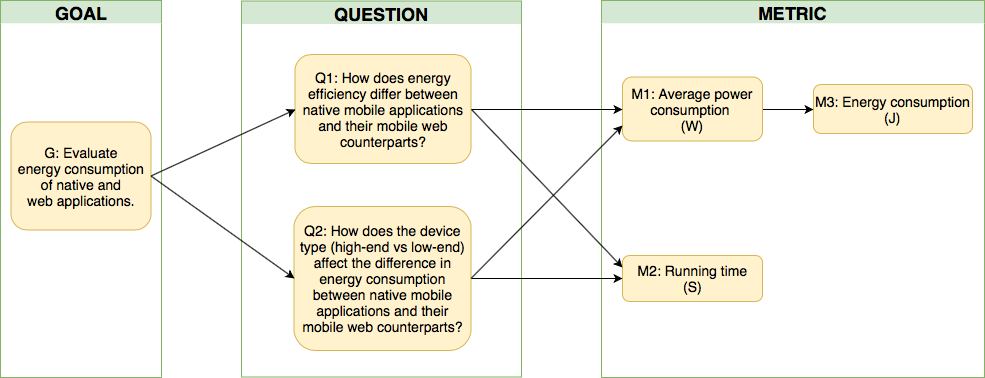
\includegraphics[width=\textwidth]{AppVSweb/figures/GQMtree.png}
%\caption{GQM model hierarchical structure}
%\label{fig:GQMtree}
%\end{figure}

\limit{2}

